\documentclass[a4paper,12pt]{article}
\pagestyle{headings}
\usepackage[utf8]{inputenc}
\usepackage{aeguill} 
\usepackage{wrapfig}
\usepackage{graphicx}
\usepackage{gensymb}
\usepackage{fullpage}
\usepackage[ngerman]{babel}
\graphicspath{ {project_proposal_img/} }
 

\begin{document}

\begin{titlepage}
\begin{center}

% Upper part of the page. The '~' is needed because \\
% only works if a paragraph has started.
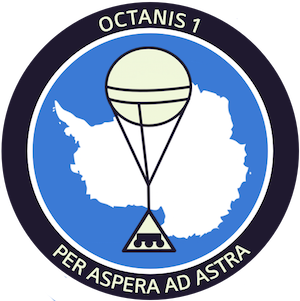
\includegraphics[width=0.35\textwidth]{patch}~\\[2cm]

\textsc{\Large Projektvorschlag}\\[0.5cm]

% Title
\huge \bfseries Octanis 1: Ein autonomer low-cost Rover für die Antarktis mit satellitengestützter Datenübertragung \\[0.4cm] 

\vspace{23pt}

\includegraphics[width=0.25\textwidth]{black_logo} \\
\vfill

% Bottom of the page
{\large \today} \\
\textsc{\small info@octanis.org | www.octanis.org}
\vspace{50pt}


\begin{table}[h!]
\centering
\vspace{1pt}
\begin{tabular}{ l  l  l }
	\textbf{Revisionen} & \textbf{Änderungen} & \textbf{Autoren} \\
	25.6.14 & Englische Originalfassung & Sam Sulaimanov, Raffael Tschui, \\ & & Ana Roldán, Pamela Canjura \\
	27.6.14 & Spanische Verison & Ana Roldán \\
	27.6.14 & Deutsche Version & Raffael Tschui \\
\end{tabular}
\end{table}

\end{center}
\end{titlepage}

\tableofcontents

\pagebreak

\section{Einführung}
»octanis | discovery and exploration« \cite{octanis} ist ein ambitiöses und herausforderndes Projekt, initiiert durch eine interdisziplinäre Gruppe von Studenten. Octanis 1 ist unsere erste Mission mit dem Ziel, einen günstigen, autonomen Roboter zu bauen der sich in polaren, schnee- und eisbedeckten Regionen bewegen kann. In einem ersten Schritt spezialisieren wir den Roboter für Wetterbedingungen der küstennahen Gebiete der Antarktis. Der Roboter wird Daten wie Temperatur, Luftdruck, relative Luftfeuchtigkeit, aktuelle Position und Lage übertragen können. Optische Sensoren an Bord werden Hindernisse erkennen und Fotos der näheren Umgebung machen können. Weitere spezifischere Datensammlung ist durchaus möglich, muss aber wegen der Energie- und Platzbeschränkungen speziell geprüft werden. Beispiele dafür sind die Konzentration eines bestimmten Gases in der Atmosphäre, $\alpha, \beta, \gamma$ Strahlung oder die Entnahme von Schnee- oder Eisproben. \\
Als eine geeignete erste wissenschaftliche Mission für Octanis 1 \cite{krishnakant} bestimmten wir die regelmässige Bodenentnahme von Schnee und Eis. Der Roboter wird mit einem kleinen Bohrkopf ausgestattet sein, welches ihm ermöglicht, in die Oberfläche zu bohren, den Schnee oder das Eis zu schmelzen und schliesslich dessen pH-Wert bestimmen.\\ 
Die Energie für Octanis liefern die Solarzellen auf seiner Oberfläche, welche die Sonnenenergie in Strom umwandeln und in einer Batterie speichern können. Dank dem Iridium Satellitennetzwerk \cite{iridium}, welches eine günstige, energieeffiziente und zuverlässige Datenübertragung bereitstellt, ist es uns möglich, mit dem Roboter jedem Punkt der Erde zu kommunizieren.


\section{Überblick}

Das Ziel der Mission Octanis 1 ist eine günstige Roboterplatform zur Verfügung zu stellen, welche nur kleine Auswirkungen auf die Umwelt hat und sich für wissenschaftliche Experimente in einer sehr kalten Umgebung eignet. Der Roboter wird so klein und leicht sein, dass er mit einem Wetterballon transportiert werden kann und seine Bauweise ermöglicht es ihm, eisiges Gelände zu durchqueren und gleichzeitig windresistent zu sein. Dank Solarzellen wird er alle nötige Energie selbst generieren und kann somit seine interne Temperatur regulieren, was sich als überlebenswichtig herausstellt. Die Platform des Roboters bekommt vier Räder, die allesamt 

*****????????????????????????... being on a controllable strut, allowing it to drive in any orientation and right itself should it flip over. 


\subsection{Ziele}

\paragraph{Robotik}
Es soll ein allwettertauglicher Leichtbauroboter entstehen mit einem einfachen, aber robusten Hardware- und Softwaredesign. Der Roboter muss die Mission grösstenteils autonom zu Ende führen können mit Eingriffen nur da wo sie nötig sind. Eine Mission enthält einen abzufahrenden Pfad und auszuführende Messungen. Über das Internet können Unterbrech- oder Hilfskommandos zum Roboter gesendet werden. Energie soll so erzeugt und gespeichert werden um dem Roboter zu ermöglichen eine Mission während mehrerer Monate ohne menschliches Zutun ausführen zu können.

\paragraph{Sensorik}
An Bord des Roboters befinden sich Messgeräte, welche regelmässig den Status der inneren und äusseren Umgebung speichern und übertragen können. Die standardisierten Schnittstellen werden es ermöglichen, wissenschaftliche Instrumente einfach ein- und auszubauen. Sämtliche übertragenen Daten von und zum Roboter werden öffentlich in Echtzeit im Internet abrufbar sein. Eine spezifische Schnittstelle wird es ihm erlauben, mit zukünftigen Robotern in einem Sensornetzwerk zu kommunizieren und als Schwarm zu funktionieren.

\paragraph{Deployment}
Es werden verschiedene Möglichkeiten den Roboter in die Antarktis zu befördern evaluiert, deren Kosten und Risiken abzuwägen sind.



\paragraph{Offen \& Reproduzierbar} 
Wir bauen Octanis in Anlehnung an die Open Source Bewegung. Sämtliche Dokumentation, Software und 3D-Modelle sind auf unserer Website zum Download verfügbar, so dass sie jede(r) wiederverwenden, verändern und verbessern kann. Wir verwenden, wo immer möglich, einfach zu beschaffende Bauteile damit jede(r) mit den nötigen Kenntnissen seine/ihre eigene Version von Octanis bauen kann. Von uns verwendete Fabrikationstechniken wie 3D-Druck sind mehr und mehr verbreitet und stehen in sogenannten Fab Labs \cite{fablab} oder Hackerspace \cite{hackerspace} einem breiten Publikum für wenig Geld zur Verfügung.
 

\subsection{Zeitplan}

Hier genannte Daten gelten für das Jahr 2014 falls nicht anders deklariert. Die genauen Daten für die wissenschaftliche Mission werden noch in Übereinstimmung mit der kooperierenden Antarktisbasis bestimmt. Das Projekt wird transparent und agil geführt und der Entwicklungsprozess ist zyklisch damit Änderungen sofort mit eingebaut werden können wenn sie nötig werden. Diese Methode konnte sich in der Vergangenheit als erfolgreich beweisen weil Fehler schnell korrigiert und die Kosten tief gehalten werden konnten. Transparenz wird dadurch geschaffen, dass die gesamte Dokumentation auf unseren öffentlichen GitHub \cite{octanisgithub} Repositories vorhanden ist. %TODO: mention live-reporting and blogging here%

\begin{table}[h!]
\centering
\begin{tabular}{ l | l | l | c }

\bfseries{Code} & \bfseries{Projektphase} & \bfseries{Daten} & \bfseries{Wochen} \\
\hline
A1 & Prototyp Design \& Entwicklung & 1.6. - 1.10. & 12 \\
A2 & Software Entwicklung & 1.6. - 1.10. & 12 \\
B1 & Erste Tests & 1.10. - 14.10. & 2  \\
B2 & Testfahrt \& Bohrtests auf Schweizer Gletscher & 14.10. - 14.11. & 4 \\
D & Mechanische Stresstests & 14.11. - 21.12. & 1 \\
E & Tests Energiemanagement & 21.11. - 14.12. & 3 \\
F & Fallschirmtests & 14.12. - 21.12. & 1 \\
0.1 & Mögliches Deployment in der Antarktis & 14.2.2015 &  1 \\
0.2 & Mögliches Deployment in der Antarktis & 1.12.2015 &  1 \\

\end{tabular}
\caption{Zeitplan Entwicklungsphasen}
\end{table}

Nach dem Abwurf des Roboters in die Antarktis wird das Wissenschaftsprojekt wie in der folgenden Tabelle beschrieben weitergeführt. Zu beachten ist, dass während der gesamten Mission eine Satellitenverbindung zum Roboter besteht, womit mehrmals täglich Statusinformationen und Messdaten übertragen werden. Um den Verlauf der Mission zu beeinflussen können jederzeit Kommandos gesendet werden.


\begin{table}[h!]
\centering
\begin{tabular}{ l | l | c }
\bfseries{Code} & \bfseries{Projektphase} & \bfseries{Wochen} \\
\hline

0 & Deployment & 1 \\
1 & Check der Systeme & 1 \\
2 & Fahrt und Probenentnahme & 3 \\
3 & Kameratests \& Bildübertragung & 3 \\
4 (*)& Test der Amateurfunk-Datenübertragung  & 3 \\

\end{tabular}
\caption{Zeitplan Wissenschaftsprojekt}

*Je nach Abwurfort des Roboters variiert der Funkkontakt zur Antarktisbasis. 

\end{table}

\pagebreak

\subsection{Team}

Wir sind eine Gruppe Studenten, die ihre Fähigkeiten bis an ihre Grenzen herausfordern. Octanis 1 wird nicht nur von uns gebaut werden, sondern mit der Hilfe vieler Professoren und Ratgebern, die wir im Verlauf des Projektes antreffen werden. Die nachfolgende Präsentation stellt deshalb das Kernteam vor:




\paragraph{Sam Sulaimanov} 
\begin{wrapfigure}{l}{0.2\textwidth}
    \centering
    \vspace{-13pt}
    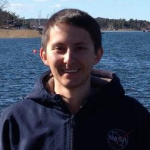
\includegraphics[width=0.15\textwidth]{sam}
\end{wrapfigure} besitzt sieben Jahre Arbeitserfahrung als Programmierer und Network Engineer. Seit jungen Jahren tüftelt er mit Mikrokontrollern und Elektronik herum und wird sicherstellen, dass Octanis' Gehirn korrekt funktionniert.
\\ \\

\begin{wrapfigure}{l}{0.2\textwidth}
    \centering
    \vspace{-13pt}
    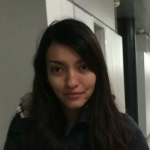
\includegraphics[width=0.15\textwidth]{ana}
\end{wrapfigure}
\paragraph{Ana Roldàn} ist eine leidenschaftliche angehende Physikerin und in allen Bereichen des Projektes involviert. Sie ist nie zu scheu, die grossen Fragen zu stellen, und inspiriert alle anderen mit ihrer grossen Leidenschaft für die Wissenschaft.
\\ \\

\begin{wrapfigure}{l}{0.2\textwidth}
     \centering
     \vspace{-13pt}
    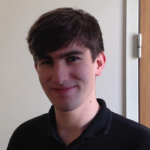
\includegraphics[width=0.15\textwidth]{raf}
\end{wrapfigure} 
\paragraph{Raffael Tschui} besitzt einen Bachelor in Elektrotechnik der EPFL und kümmert sich um die lebenswichtige Energieversorgung und -verwaltung des Roboters. Im Moment arbeitet er zusammen mit einem EPFL Professor an einem Projekt in Kolumbien, in dem er beim Bau eines wasserreinigenden Bioreaktor mitwirkt.  
\\ \\

\begin{wrapfigure}{l}{0.2\textwidth}
    \centering
    \vspace{-13pt}
    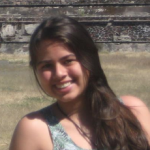
\includegraphics[width=0.15\textwidth]{pam}
\end{wrapfigure} 
\paragraph{Pamela Canjura} interessiert sich seit sie fünf Jahre alt war für Chemie und nimmt regelmässig an der Chemie Olympiade teil. Sie befasst sich mit den chemischen Analysen, welche an Bord von Octanis gemacht werden können.
\\ \\


\subsection{Budget}

Tabelle 3 listet die geplanten Kosten auf mit einer Toleranz von $\pm 20\%$ (krit. = Missionskritisch). \\ 

\begin{table}[h!]

\centering
\begin{tabular}{ l | c || r }
  Beschreibung & Priorität & Einmalige Kosten \\
  \hline
  Roboter Solar \& Heizung & krit. & 1000 CHF \\
  Roboter Kommunikation & krit. & 500 CHF \\
  Roboter Instrumente \& Sensoren & krit. & 500 CHF \\
  Roboter Elektronik & krit. & 700 CHF \\
  Roboter Mechanik \& Mobilität & krit. & 1000 CHF \\
  Ballon Transport & opt. & 1500 CHF \\
  \hline \hline
  & & kritisch: 3700 CHF  \\
  & & optional: 1500 CHF \\
\end{tabular}
\caption{Allgemeines Budget.}
\end{table}

Die einzigen wiederkehrenden Kosten werden von der Iridium Satellitenübertragung \cite{iridium} verursacht. Diese reichen von 0.04-0.12 GBP pro Nachricht (340 bytes für ausgehende Nachrichten) zuzüglich der Verbindungsmiete von 8 GBP pro Monat. Der Preis einer Nachricht hängt von der Anzahl benötigten Nachrichten ab.



\section{Rover Transport und Deployment}

Octanis 1 ist ein Leichtbau-Roboter mit einem Endgewicht von nicht mehr als 2.5kg. Dank dieser Bauweise kommen mehrere kosteneffiziente Deployment-Methoden in Frage, die hier aufgeführt sind: 

\subsection{Deployment-Methoden}

\begin{figure}[h!]
	\centering
    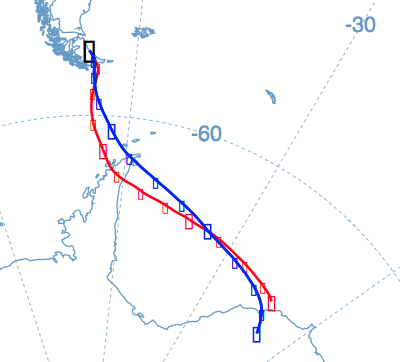
\includegraphics[width=0.4\textwidth]{trajectory}
    \caption{HYSPLIT trajectory simulation starting in Rio Grande, Argentina.} %TODO%
\end{figure}

\paragraph{Stratosphären-Ballons} auch als Wetterballone bekannt, können benutzt werden um den Roboter zu seinem Zielort zu transportieren. Helium-gefüllt erreichen diese Ballone normalerweise eine Höhe von 30km und können hunderte von Kilometer überwinden. Allerdings kann der Pfad des Ballons nicht beeinflusst werden und setzt eine gute und ausgiebige Flugpfad-Simulation voraus. Diese Simulationen können mit der HYSPLIT Simulationssoftware \cite{hysplit} \cite{hysplitjava} durchgeführt werden. Das ist eine günstigste Methode um den Rover in der Antarktis zu deployen, denn man braucht nur in den südlichste Region Südamerikas zu reisen, wo kommerzielle Fluggesellschaften hinfliegen. Von dort kann man den Ballon auf einen Luftpfad bringen, der in die Antarktis führt. Mit all den Vorteilen kommt ein höheres Risiko, dass das Deployment nicht funktioniert. Auch mit guten Wettermodellen, bleibt das Wetter unberechenbar und eine plötzliche Änderung könnte den Ballon vom Pfad abbringen. HYSPLIT wurde aber schon erfolgreich in anderen Ballon-Projekten eingesetzt wie z.B. beim Breitling-Orbiter 3 Projekt von Piccard und Jones \cite{hysplitexamples}.
Sobald der Ballon über dem Ziel schwebt kann der Roboter abgetrennt werden, welcher mit dem Fallschirm landet. Der Ballon wird danach unkontrollierbar weiterschweben bis er platzt oder aber auf die Erde zurückfällt nachdem das Helium herausdiffundiert.

\begin{figure}[h!]
	\centering
    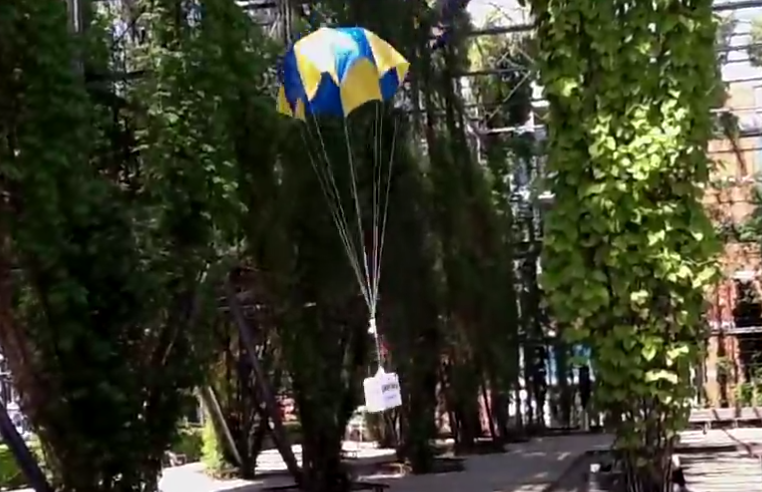
\includegraphics[width=0.5\textwidth]{lowcostchute}
    \caption{Ein von uns produzierter low-cost Fallschirm im Test. }
\end{figure}


\paragraph{Helikopter} - eine etwas andere Art Octanis zu deployen ist mit einem Helikopter der eine feste Route fliegt (Personen- oder Warentransport) fliegt. Der Roboter könnte einem Passagier gegeben werden oder an die Transportleine des Helikopters befestigt werden um ihn im Flug abzuwerfen. Gleich wie bei der Ballonmethode schwebt Octanis mit einem Fallschirm zu Boden und kann seine Mission beginnen.


\paragraph{Manuelles} deployment ist empfohlen wenn Kosten und Risken so tief wie möglich gehalten werden sollen. Das ist die einfachste Methode den Roboter zu seinem Erkundungsort zu bringen, denn man muss ihn einfach selber dorthin bringen. Typischerweise direkt bei der Basis oder ein paar Kilometer entfernt. Octanis kann seine Mission beginnen und zum Startort zurückfahren.




\subsection{Environmental Sustainability}
It is desirable to not leave any waste behind as well as it is required by the Antarctic Treaty. Depending on the method of deployment, the total mass and types of materials that will be included on a mission to Antarctica vary. A deployment of the rover to a target out of reach of normal Antarctic expeditions is done by using a High Altitude Balloon or a standard 3kg latex weather balloon. In such a long-distance mission, the rover will be separated from the balloon at the target location and the balloon will continue to fly unattended. Therefore the landing location of the balloon can not be known. Due to the nature of such a long-distance mission, typically the rover is unreachable to any expedition or base - the rover is left for the benefit of information on that location.

In a first step, it is therefore proposed to select a landing site that is in reach of normal Antarctic expeditions or bases. It is even possible to release the rover by other means like bringing it to the location manually or via helicopter.

Concluding, the rover is a construction of various polymers and metals, and a small risk exists that it will end up being uncontrollable due to malfunction. The total rover mass however does not exceed 2.5kg and therefore the pollution produced is small. In the unlikely event of failure, the rover can then be retrieved manually thanks to the last known transmitted location.




\section{Rover Subsystems}

\subsection{Board Computer}
\begin{figure}[h!]
	\centering
    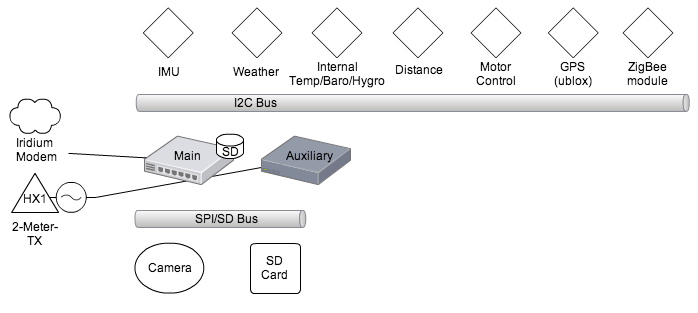
\includegraphics[width=1\textwidth]{schema}
    \caption{Schema of the on-board computing system with peripherals.}
\end{figure} 
The Texas Instruments MSP430 16-bit ultra-low power microcontroller family is the preferred processor choice for the embedded computer system of the rover. The microcontroller will take over most control and regulation tasks, specifically driving, navigation, communications and sensor processing. The system will run a realtime operating system capable of reliably multitasking with prioritised tasks. The computer will interact with the following on-board peripherals:

\begin{itemize}
\item Inertial Measurement Unit: accelerometer, gyroscope, magnetometer, precision barometer.
\item Weather module: temperature, barometer, hygrometer, anemometer.
\item Science instrument: pH probe.
\item Optics module: camera, distance sensors.
\item Drive module: motor controllers, current sensors.
\item Communication: Iridium, APRS, ZigBee.
\item SD card memory.
\item GPS module.
\end{itemize}

An auxiliary computer will take over if the main computer malfunctions. It will try to reset the main computer and if unsuccessful provide basic system functionality.



\subsection{Power}

The energy of the sunlight per square meter is $E_0*sin(\alpha)$ with $E_0=1367 W/m^2$ \cite{solarc} and $\alpha$ the angle between the direct incoming sunrays and the horizontal. For the Antarctic, we can use $\alpha \approx 23.5+90+|\phi|$ where $\phi$ is the latitude, to get an estimate of the maximum energy (i.e. in summer) at a certain geographic point (see fig. 4).


\begin{figure}[h!]
	\centering
    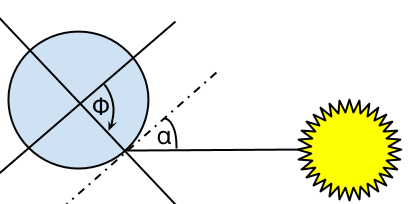
\includegraphics[width=0.6\textwidth]{sun}
    \caption{Octanis rover design concept built after MUSES-CN nanorover.}
\end{figure}


 This would lead to $1050 W/m^2$ for the northmost point of the antarctic (@ 65\degree S) and $545 W/m^2$ at the south pole (@ 90\degree S). Bare in mind that, during the six sunny months this value will oscillate between 0 and the maximum value just calculated \cite{pvedu}. 
Assuming our panels are installed horizontally and considering current solar panel efficiency (around 15-20\%) this means that per square meter we can convert max. 200 W into electrical energy. If we take a pessimistic efficiency and a “radiation mean value” during the 6 months of the mission (just 1/2 of the maximum value) we would need a panel of the size of $0.13m^2$ (@ 65\degree S) to $0.25m^2$ (@ 90\degree S) to output a power of 10 W. But, this didn’t consider the daily oscillation of the radiation angle, nor that it does get night during certain time periods for any point north from the south pole. Therefore, it is more reasonable to take the pessimistic $0.25m^2$ value (also because the energy supply will decrease with bad weather).

To summarise, a panel surface of $0.25m^2$ will provide us with an average (seasonal, daily) power of 10W and these numbers are proportional. 


\subsection{Thermal}

The ultimate priority is to keep the system at -20\degree C or above, which means that all the energy from the solar cell and, if necessary, from the battery will first be used to maintain this goal. The heating system is therefore directly connected between the solar cell and the battery charge controller. It is controlled with electronic comparators that enable one or another energy source to power the heating pads depending on temperature thresholds listed below. The charge controller itself takes care of the temperature limits for charging the battery and switches itself on and off automatically. 


\subsection{Mechanical}
The rover body design (fig. 5) has been substantially influenced by NASA's MUSES-CN nanorover \cite{muses}. The nanorovers design is a unique design as it allows almost complete freedom. We have designed Octanis 1 to be lightweight with a large enough surface area to produce enough solar energy for the mission duration. The body dimensions are roughly 30cm x 30cm x 6cm.

\begin{figure}[h!]
	\centering
    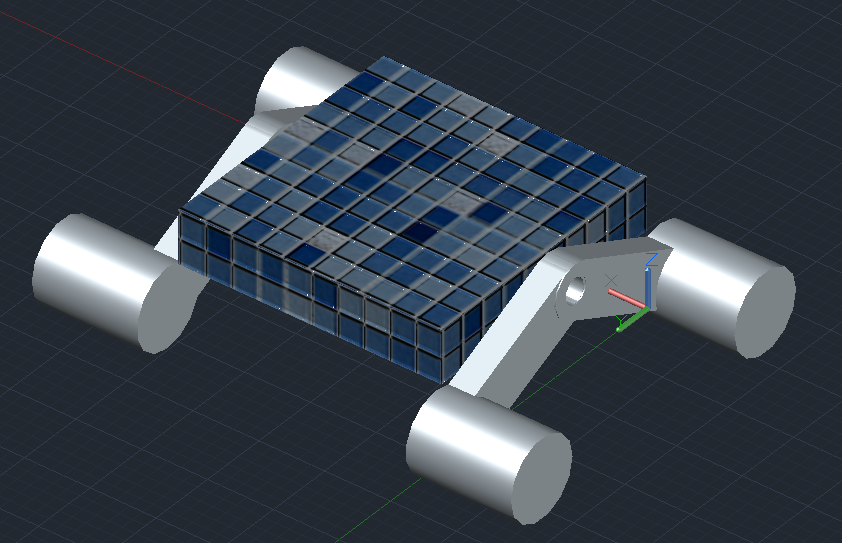
\includegraphics[width=0.5\textwidth]{conceptrover}
    \caption{Octanis rover design concept built after MUSES-CN nanorover.}
\end{figure}

As depicted in figure 6, this rover design allows many orientations for different situations. Main concerns of the mission are energy supply and weather resistance. As the whole rover body is covered with solar cells, the rover can right itself up according to sun position to expose most of its area to sunlight. In harsher weather conditions it is also crucial to make sure snow doesn't cover up the panels. This can be prevented by periodically flipping the rover. Not only snow, but wind can be an issue and sometimes even flipping over the rover. If this occurs, the rover can return to a driving position by actuating the struts. All wheel struts can be rotated around the axis and are fitted with a separate motor each. They are moved through a worm drive to keep them static when they are not rotating without having to apply constant power. \\
Another benefit of this design is it allowing us to build a simpler drilling device. When drilling an ice core, the rover can lower itself to the ground exploiting its own weight as pressure onto the drill. The drill bit just needs to spin and doesn't need to retract into the rover body.

\begin{figure}[h!]
\centering
\begin{tabular}{ c  c  c }
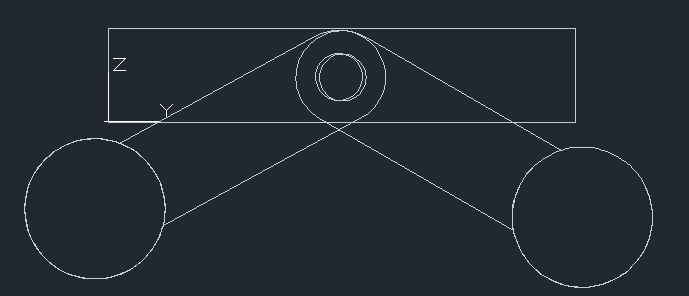
\includegraphics[width=0.3\textwidth]{drive} & 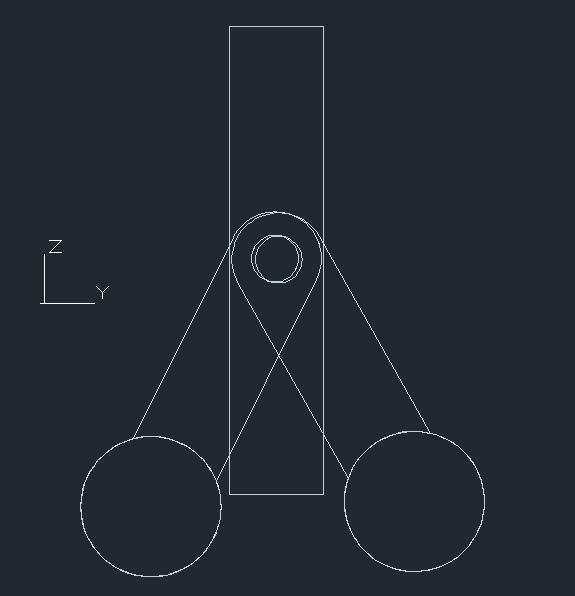
\includegraphics[width=0.25\textwidth]{upright} & 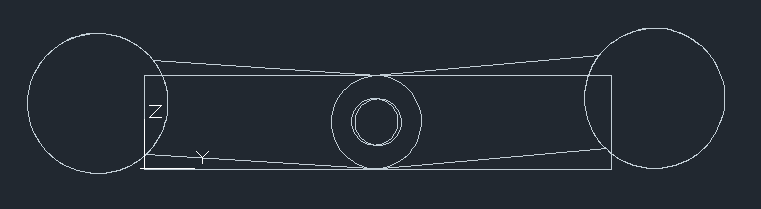
\includegraphics[width=0.4\textwidth]{flat} \\
\end{tabular}
\caption{Different wheel strut configurations l.t.r.: (1) drive mode, (2) solar recharge mode, (3) wind protect mode.}
\end{figure}


\subsection{Mobility}
Snowy and icy terrain will be Octanis' main habitat and so its wheels need to be specifically designed to be wide, lightweight and should provide a good traction going upwards. 
All four wheels will be individually motorised and provide enough torque to move Octanis on an inclination of 30 degrees. Turning can be achieved by rotating the wheels on each side at different speeds. 

\begin{figure}[h!]
	\centering
    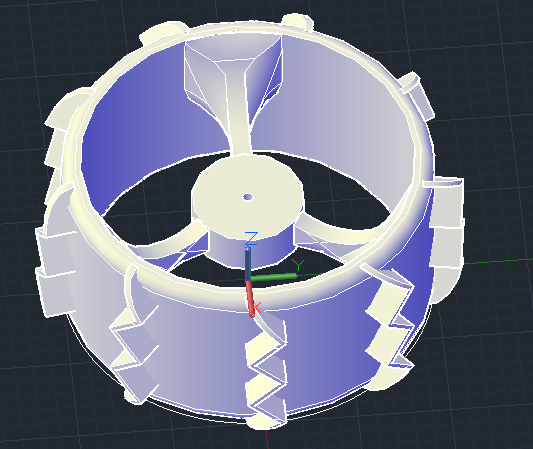
\includegraphics[width=0.4\textwidth]{wheel}
    \caption{Initial wheel design. Fins allow the wheel to dig into the snow while driving providing better traction.}
\end{figure}


An inertial measurement unit (IMU) will be used to know the rovers orientation at any point in time. It consists of a gyroscope, accelerometer, precision barometer and magnetometer. The sensors information is fed back to the control systems that actuate the motors. Should the rover need to go over an obstacle, the wheel struts will be rotated as far as possible so that the rover body is always in a plane parallel to the ground. This minimises the risk of being tipped over and should allow the easy traversal of obstacles higher than the wheel radius and is similar to the rocker-bogie suspension system used on NASAs mars rovers \cite{rockerbogie}. Due to the high risk of overturn caused by wind gusts the passive rocker-bogie design was not chosen, since there would be no simple way of righting back up.

Octanis' top speed is estimated to be at 100cm/min. Disregarding energy availability depending on weather, gives it a daily range of around 1km. There will be two driving modes: discovery and shortest path. \textbf{Discovery mode} will make the rover densely traverse either a preprogrammed circular area of a map or on detecting a certain phenomena (e.g. higher pH levels). \textbf{Shortest path} brings Octanis from waypoint to waypoint using the shortest path. Both methods can be used in combination. Detected obstacles can be stored as landmarks and help build a rough map.

\subsection{Communication}
Regular data transmission is a mission critical feature of the rover. It is achieved by using the Iridium Short Burst Data (SBD) service with the help of the RockBLOCK Iridium 9602 modem \cite{iridium}. This modem allows the transmission of data packets of up to 340 bytes outwards and 270 bytes inwards approximately every 20 seconds. Larger data frames can be fragmented and transmitted with multiple packets. The key to this modem and network is that is available everywhere on Earth at any time, something that cannot be said of the GSM network or even amateur radio. That the modem require just as low power as the GPS on board adds to the list of benefits. Information sent through the Iridium network is automatically sent to a server and uploaded to the project website, where the public can view Octanis' state and data.

Octanis 1 will also be equipped with a 5 watt one-way APRS transmitter, transmitting sensor data and location information on the 2-meter band. This can be received by amateur radio operators (or unlicensed individuals with radio scanners) who are in range. The range of this transmitter is typically hundreds of kilometers when travelling in the sky (i.e. attached to a balloon). On the ground, the range is orders of magnitude smaller.


\subsection{Optical}
Octanis will be able to take snapshots on-demand with a low resolution camera. It is part of an experiment to find out if an image can be efficiently sent via the Iridium network. Additionally we would like to test on-board image processing (e.g. simple feature detection). The optical system is completed by distance sensors that can detect nearest obstacles. It will be evaluated if the Neato XV-11's LIDAR \cite{lidar} can be used or if we should proceed with IR distance sensors.


\subsection{Scientific Instrument}
The preferred scientific instrument for this mission is a ice core drill combined with a pH probe. The drill is able to drill a small 1cm x 5cm ice/snow core, retract it from the cold surface and then melt the sample. The ice/snow-water can be analysed with a pH probe, that is typically a glass electrode, to determine the pH value. Due to the low-cost nature of the sensor to be used, precision cannot be guaranteed by the manufacturer and has to be calibrated and tested by us. It is though assumed that the device will give good readings for comparison of a high quantity of samples.

\pagebreak

\section{Conclusion}
Knowing that this mission is an ambitious one and will have many challenges to be solved on the way, we believe that it is a possible and viable project. When we can achieve our objectives, we will be able to provide the scientific community (including so-called citizen scientists) with a universal and adaptable rover platform. Proving ourselves in the harsh environment of Antarctica means that our rover can survive many other similar environments. \\

We hope to fascinate and inspire students, teachers, artists, entrepreneurs, scientists - in the end all people - for interdisciplinary research, engineering and knowledge sharing, hoping that they will join us on the grand mission to a better world!


\pagebreak
\pagestyle{empty}
\begin{thebibliography}{1}


\bibitem{krishnakant}
  Krishnakant Babanrao Budhavant, Pasumarthi Surya Prakasa Rao, Pramod Digambar Safai,
  \emph{Chemical Composition of Snow-Water and Scavenging Ratios over Costal Antarctica}.
  Aerosol and Air Quality Research, 14: 666–676, 2014.

\bibitem{octanis}
{\em »octanis | discovery and exploration« website} http://octanis.org, 23.6.2014.

\bibitem{iridium}
{\em Rock7 RockBLOCK website} http://rockblock.rock7mobile.com/products-rockblock.php, 25.6.2014.


\bibitem{octanisgithub}
{\em Octanis 1 GitHub repositories website} http://github.com/octanis1, 25.6.2014.

\bibitem{muses}
  Brian H. Wilcox, Ross M. Jones, 
  \emph{The MUSES-CN Nanorover Mission and Related Technology}.
  IEEE Aerospace 2000 Conference, 18.3.1999.


\bibitem{rockerbogie}
  Hayati, S., et. al., 
  \emph{The Rocky 7 Rover: A Mars Sciencecraft Prototype}.
  Proceedings of the 1997 IEEE International Conference on Robotics and Automation, pp. 2458-64, 1997.

\bibitem{hysplit}
  {\em HYSPLIT - Hybrid Single Particle Lagrangian Integrated Trajectory Model }, NOAA, http://www.ready.noaa.gov/HYSPLIT.php, 23.6.2014.

\bibitem{hysplitjava}
  {\em JAVA software to run multiple HYSPLIT simulations to find the optimal parameters for a trajectory}, http://github.com/octanis1/OctanisHYSPLIT, 23.6.2014.

\bibitem{hysplitexamples}
	{\em Ballooning with HYSPLIT}, \\
	http://www.arl.noaa.gov/documents/workshop/Spring2010/Balloon\_flights.ppt, 23.6.2014.

\bibitem{fablab}
	{\em Fab lab definition}, \\
	http://en.wikipedia.org/wiki/Fab\_lab, 25.6.14.

\bibitem{hackerspace}
	{\em Hackerspace definition}, \\
	http://en.wikipedia.org/wiki/Hackerspace, 25.6.14.

\bibitem{pvedu}
	{\em Effect of Light Intensity}, \\
	http://www.pveducation.org/pvcdrom/solar-cell-operation/effect-of-light-intensity, 25.6.14.

\bibitem{lidar}
	{\em Neato XV-11 LIDAR / Piccolo Laser Distance Sensor}, \\
	http://xv11hacking.wikispaces.com/LIDAR+Sensor, 25.6.14.

\bibitem{solarc}
	{\em Solar constant}, \\
	http://en.wikipedia.org/wiki/Solar\_constant, 25.6.14.

\end{thebibliography}

\end{document}